\documentclass{rapportProjetSI2024}



\addbibresource{biblio.bib}

%--------------------------------------

\titre{Rapport sur Projet TP SI : L3 ISIL A}
\soustitre{Conception et Réalisation d’un Système d’Information pour la Gestion des
Ressources Humaines (RH) d’une Entreprise.}

\enseignant{Rachid \textsc{Boudour} \\}

\eleves{Ilyes \textsc{Medjedoub} \\
	Asma \textsc{Touafek} \\ 
	Mohamed Amine \textsc{Belhadji} }

%--------------------------------------

\begin{document}

\fairepagedegarde
\fairetabledesmatieres

%--------------------------------------

\section{Gestion des Favoris}

\subsection{Description}
L'agent RH pourra choisir des fonctionnalités pour un accès rapide.

\subsection{Conception Logique}

\subsubsection{Diagramme de Cas d'Utilisation}
\begin{figure}[H]
    \centering
    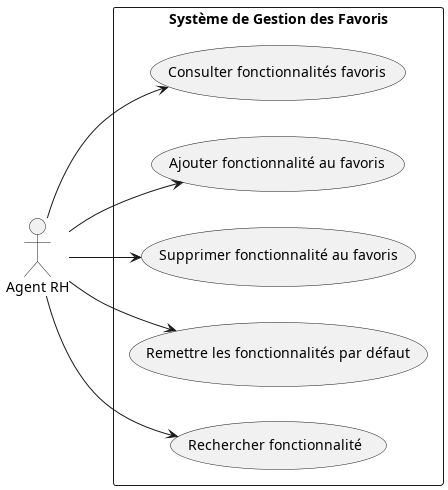
\includegraphics[width=0.5\textwidth]{usecase/gestion-favoris-usecase.png}
    \caption{Diagramme de Cas d'Utilistion: Gestion des Favoris.}
    \label{fig:gestion-favoris-usecase}
\end{figure}

\subsubsection{Modèle Conceptuel de Donnée}
\begin{figure}[H]
    \centering
    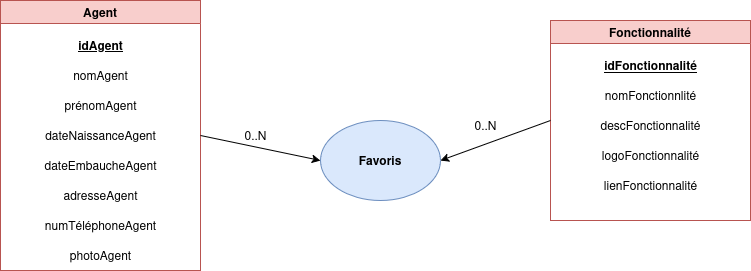
\includegraphics[width=1\textwidth]{mcd/gestion-favoris-mcd.png}
    \caption{Modèle Conceptuel de Donnée: Gestion des Favoris.}
    \label{fig:gestion-favoris-mcd}
\end{figure}

\subsubsection{Modèle Logique de Donnée}
\begin{itemize}
    \item \textbf{Agent} (\underline{idAgent}, nomAgent, prenomAgent, dateNaissanceAgent, dateEmbaucheAgent, adresseAgent, numTelephoneAgent, photoAgent)
    \item \textbf{Favoris} (\underline{idAgent*, idFonctionnalite*})
    \item \textbf{Fonctionnalite} (\underline{idFonctionnalite}, nomFonctionnalite, descFonctionnalite, logoFonctionnalite, lienFonctionnalite)
\end{itemize}

\subsubsection{Diagramme de Classes}
\begin{figure}[H]
    \centering
    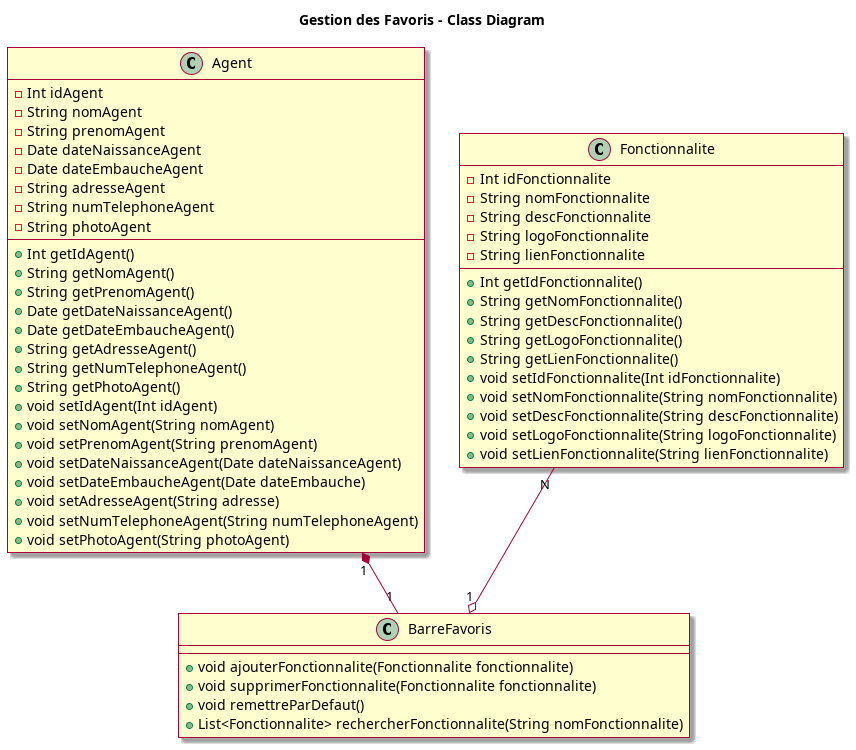
\includegraphics[width=1\textwidth]{classes/gestion-favoris.png}
    \caption{Diagramme de Classes: Gestion des Favoris.}
    \label{fig:gestion-favoris-classes}
\end{figure}

\subsection{Conception Graphique}
\lipsum[8]

\subsection{Manuel d'Utilisation}
\lipsum[9]

\section{Section 2}
\lipsum[5]

\section{Des commandes utiles}

\textbf{Insérer une image}
\begin{figure}[H]
    \centering
    
\includegraphics[width=0.5\textwidth]{logos/logo.png}
    \caption{Insérer une image.}
    \label{fig:logo}
\end{figure}

ou la version raccourcie avec \texttt{\textbackslash insererfigure} : \insererfigure{logos/logo.png}{0.5\textwidth}{Insérer une image avec une commande.}{logo_raccourci}


\textbf{Citer une figure} avec \texttt{\textbackslash ref} : \ref{fig:logo_raccourci}.\\


\textbf{Insérer des expressions mathématiques} en bloc :
\begin{equation*}
    \int_{-\infty}^{\infty} e^{-x^2} \, \text{d}x = \sqrt{\pi}
\end{equation*}

ou bien en \textit{inline} : $\int_{-\infty}^{\infty} e^{-x^2} \, \text{d}x = \sqrt{\pi}$.\\


\textbf{Insérer une série de calculs}
\begin{align*}
    x &= 0.999\ldots \\
    10x &= 9.999\ldots \\
    10x - x &= 9.999\ldots - 0.999\ldots \\
    9x &= 9 \\
    x &= 1 \\
    0.999\ldots &= 1
\end{align*}


\textbf{Insérer une liste}
\begin{itemize}
    \item Premier niveau
    \begin{itemize}
        \item Deuxième niveau
        \item Un autre élément au deuxième niveau
    \end{itemize}
    \item Un autre élément au premier niveau\\
\end{itemize}


\textbf{Insérer un tableau simple} \\
\begin{table}[H]
    \centering
    \begin{tabular}{|c|c|c|}
        \hline
        A & B & C \\
        \hline
        1 & 2 & 3 \\
        4 & 5 & 6 \\
        \hline
    \end{tabular}
    \caption{Un tableau simple.}
    \label{tab:tableau_simple}
\end{table}


\textbf{Insérer du code} : \texttt{print("Hello, World!")}.\\


\textbf{Insérer et référencer une boîte de code} : 
\hyperref[exemple_code]{Code \ref*{exemple_code}}.\\
Attention : le label (ici, \texttt{exemple\_code}) doit être écrit deux fois lors du référencement. Une fois dans le premier argument de \texttt{\textbackslash hyperref}, puis une seconde fois dans \texttt{\textbackslash ref*} :

\begin{center}
\texttt{\textbackslash hyperref[exemple\_code]\{Code \textbackslash ref*\{exemple\_code\}\}}.
\end{center}

\begin{codebox}[exemple_code]{Un exemple de boîte de code \texttt{Python}}
\begin{minted}{python}
def sieve_of_eratosthenes(n):
    '''Returns a list of all prime numbers up to n.'''
    primes = [True] * (n + 1)
    primes[0] = primes[1] = False  # 0 and 1 are not prime numbers
    for i in range(2, int(n**0.5) + 1):
        if primes[i]:
            for j in range(i * i, n + 1, i):
                primes[j] = False
    return [i for i, is_prime in enumerate(primes) if is_prime]
\end{minted}
\end{codebox}


\textbf{Citer une source} depuis \texttt{biblio.bib} avec \texttt{\textbackslash cite} : \cite{exemple_de_source}.\\


\textbf{Afficher une bibliographie} rapidement avec \texttt{\textbackslash insererbiblio}.

\insererbiblio 

\end{document}